\begin{question}
\noindent Shape $A$ and shape $B$ are drawn on the grid below.

\begin{center}
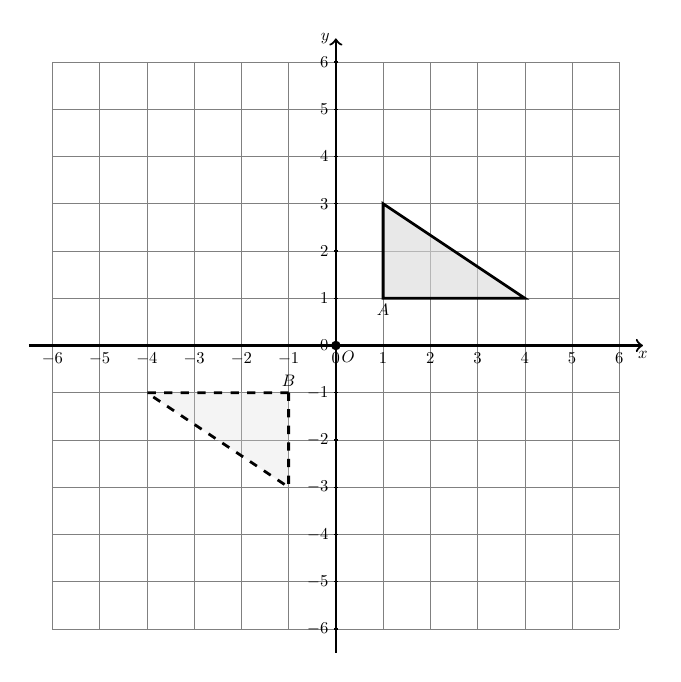
\begin{tikzpicture}[scale=0.6, transform shape]
    \def\axisLimit{6}

    \draw[step=1cm,gray,very thin] (-\axisLimit,-\axisLimit) grid (\axisLimit,\axisLimit);

    \draw[thick,->] (-\axisLimit-0.5,0) -- (\axisLimit+0.5,0) node[anchor=north] {$x$};
    \draw[thick,->] (0,-\axisLimit-0.5) -- (0,\axisLimit+0.5) node[anchor=east] {$y$};

    \foreach \x in {-\axisLimit,...,\axisLimit}
        \draw (\x cm,1pt) -- (\x cm,-1pt) node[anchor=north] {$\x$};
    \foreach \y in {-\axisLimit,...,\axisLimit}
        \draw (1pt,\y cm) -- (-1pt,\y cm) node[anchor=east] {$\y$};

    % Shape A: right-angled triangle with vertices (1,1), (4,1), (1,3)
    \coordinate (A1) at (1,1);
    \coordinate (A2) at (4,1);
    \coordinate (A3) at (1,3);
    \filldraw[fill=gray!30, draw=black, line width=1pt, fill opacity=0.6] (A1) -- (A2) -- (A3) -- cycle;
    \node[below] at (A1) {$A$};
    \node[below right] at (A2) {};
    \node[above left] at (A3) {};

    % Shape B: rotation of A by 180 degrees about (0,0)
    % (1,1) -> (-1,-1), (4,1) -> (-4,-1), (1,3) -> (-1,-3)
    \coordinate (B1) at (-1,-1);
    \coordinate (B2) at (-4,-1);
    \coordinate (B3) at (-1,-3);
    \filldraw[fill=gray!30, draw=black, line width=1pt, fill opacity=0.3, dashed] (B1) -- (B2) -- (B3) -- cycle;
    \node[above] at (B1) {$B$};

    % Mark the centre of rotation
    \filldraw[black] (0,0) circle (2.5pt);
    \node[below right] at (0,0) {$O$};

\end{tikzpicture}
\end{center}

\noindent Describe fully the single transformation that maps shape $A$ onto shape $B$.

\vspace{5cm}

\begin{flushright}
\answerlines{3}{3}
\end{flushright}
\end{question}
